\chapter{ Chapitre  5  : Sprint 2 " Gestion \centering  des Universités Endroits et des Examens"}
\begin{spacing}{1.2}
\minitoc
\thispagestyle{MyStyle}
\end{spacing}
\newpage
\begin{sloppypar} 

\section{Introduction }
\vspace{-4mm}
Le prochain sprint sera axé sur la gestion des universités, des Endroits et des examens, qui seront affichés sur l'application mobile pour tous les utilisateurs. L’objectif est de fournir à l’admin les outils nécessaires pour gérer efficacement et en toute sécurité les informations relatives aux universités, aux Endroits disponibles et aux examens.
\vspace{-9mm}
\section{Backlog du sprint}
\vspace{-4mm}
Le backlog de gestion des universités, des Endroits et des examens propose des fonctionnalités pour ajouter, modifier, supprimer et consulter ces informations dans notre application.
\vspace{-4mm}
\begin{table}[H]
\centering
\begin{tabular}{|p{11cm}|p{2cm}|p{2.5cm}|}
\hline
\textbf{ Tâches } & \textbf{ Priorité }& \textbf{Période/jour}  \\
\hline
En tant qu’un admin je peux gérer  les universités dans l’application web.  & Élevée  & 4 jours  \\
\hline
En tant qu’un admin je peux gérer les Endroits dans l’application web.   & Élevée  & 3 jours  \\
\hline
En tant qu’un admin je peux gérer les examens dans l’application web. & Élevée & 4 jours \\
\hline
En tant qu’un utilisateur je peux consulter  les universités dans l’application mobile. & Élevée  & 3 jours \\
\hline
En tant qu’un utilisateur je peux consulter  les Endroits dans l’application mobile. & Moyenne & 1 jour\\
\hline
En tant qu’un utilisateur je peux consulter  les examens dans l’application mobile. & Moyenne & 1 jour\\
\hline
\end{tabular}
\caption{Tableau de Backlog de produit Sprint 2}
\end{table}

\vspace{-1.3cm}
\section {Analyse et spécification des besoins}
\vspace{-7mm}
\subsection{Diagramme de cas d’utilisation detaillé}
\vspace{-4mm}
Afin de mieux comprendre la structure de notre système, nous avons utilisé un diagramme de cas d'utilisations qui est présenté ci-dessous.
\vspace{-4mm}
\begin{figure}[H]%
    \centering
    \setlength{\fboxsep}{5pt}%
    \setlength{\fboxrule}{0.5pt}%
    \fbox{
    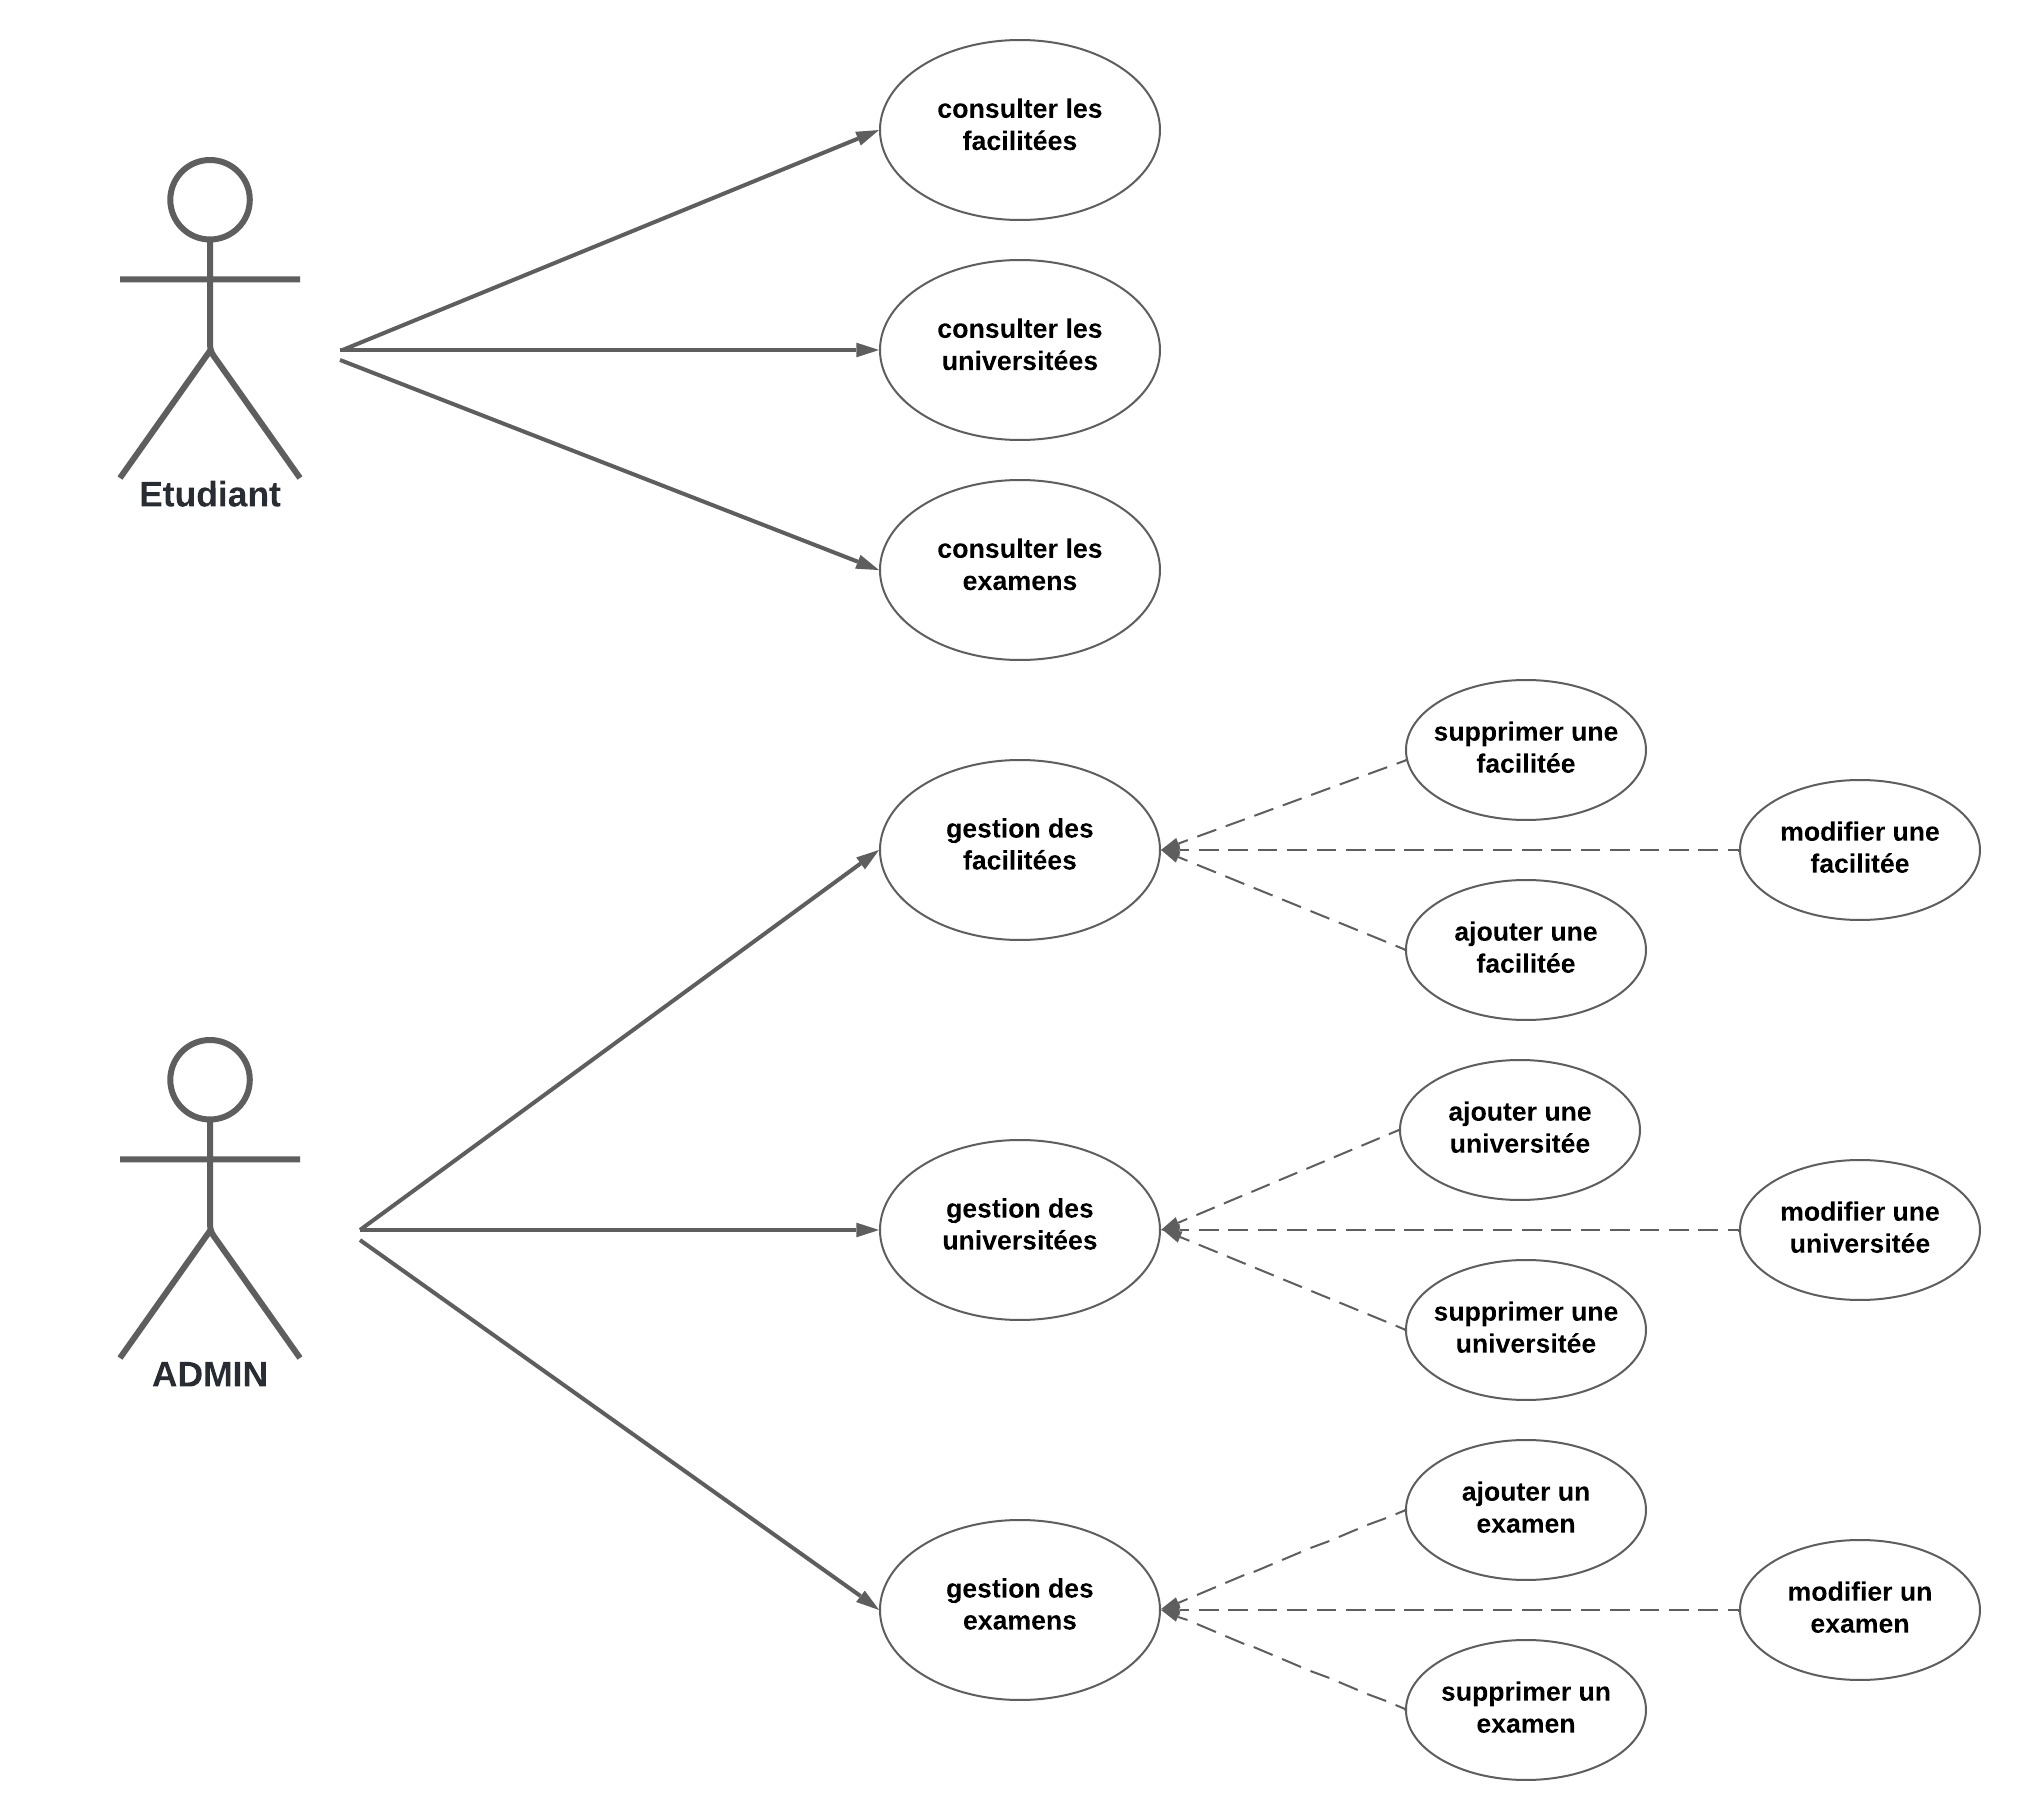
\includegraphics[height=10cm,width=15cm]{images/AAADiagrammedesCasFacUnEx.png}%
    }
    \caption{Figure du Diagramme de cas d'utilisation Sprint 2}
\end{figure}
\vspace{-1cm}
\subsection{Description textuelle du cas d’utilisation « Ajouter un endroit »}
\vspace{-3mm}
La description textuelle du cas d'utilisation "Ajouter un endroit" détaille le processus par lequel un admin peut créer un nouvel endroit sur la plateforme web de l'application, en fournissant des informations telles que le nom de l'endroit, sa localisation, sa description, etc.

\begin{table}[h]
\centering
\begin{tabular}{|p{3cm}|p{12cm}|}
\hline
\textbf{Cas d'utilisation } & Ajouter un endroit  \\
\hline
\textbf{Acteurs} & Admin \\
\hline
\textbf{Précondition} & Admin authentifié \\
\hline
\textbf{Postcondition} & endroit  ajoutée \\
\hline
\textbf{Scénario nominal} &
\begin{enumerate}
    \item Le système affiche l’interface de gestion des données.
    \item L’admin la catégorie correspondante.
    \item L'admin saisit les inforamtions necessaires .
    \item L'admin appuit sur le bouttin <<Add>>.
    \item Le système vérifie que tous les champs sont remplis. S'ils ne le sont pas, une exception est déclenchée.
    \end{enumerate} \\
\hline
\textbf{Exception } & Champs non remplis. \\
& Le système affiche un message d’erreur informant l’utilisateur que tous les champs doivent être remplis.  \\
\hline

\end{tabular}
\caption{Description du cas d’utilisation « Ajouter un endroit »}
\end{table}

\subsection{Description textuelle du cas d’utilisation « Modifier un endroit »}
\vspace{-3mm}
La description du cas d'utilisation "Modifier un endroit" décrit comment un admin peut mettre à jour les informations d'un endroit existant sur la plateforme web de l'application. Cela inclut la modification de détails tels que le nom de l'endroit, sa localisation, sa description, etc.
\begin{table}[h]
\centering
\begin{tabular}{|p{3cm}|p{12cm}|}
\hline
\textbf{Cas d'utilisation } & Modifier un endroit  \\
\hline
\textbf{Acteurs} & Admin \\
\hline
\textbf{Précondition} & Admin authentifié \\
\hline
\textbf{Postcondition} & endroit  modifié \\
\hline
\textbf{Scénario nominal} &
\begin{enumerate}
    \item Le système affiche l’interface de gestion des données.
    \item L’admin la catégorie correspondante.
    \item L'admin modifie les inforamtions  .
    \item L'admin appuit sur le bouttin <<Edit>>.
    \item Le système vérifie que tous les champs sont remplis. S'ils ne le sont pas, une exception est déclenchée.
    \end{enumerate} \\
\hline
\textbf{Exception } & Champs non remplis. \\
& Le système affiche un message d’erreur informant l’utilisateur que tous les champs doivent être remplis.  \\
\hline

\end{tabular}
\caption{Description du cas d’utilisation « Modifier un endroit »}
\end{table}
\vspace{-1cm}
\subsection{Description textuelle du cas d’utilisation « Supprimer un endroit »}
\vspace{-4mm}
La description du cas d'utilisation "Supprimer un endroit" décrit le processus par lequel un administrateur peut retirer un endroit de la plateforme web de l'application. Cela implique de sélectionner l'endroit à supprimer, puis de confirmer cette action. Une fois supprimé, l'endroit ne sera plus visible pour les utilisateurs de l'application.


\begin{table}[h]
\centering
\begin{tabular}{|p{3cm}|p{12cm}|}
\hline
\textbf{Cas d'utilisation } &  supprimer un endroit  \\
\hline
\textbf{Acteurs} & Admin \\
\hline
\textbf{Précondition} & Admin authentifié \\
\hline
\textbf{Postcondition} & endroit  supprimé \\
\hline
\textbf{Scénario nominal} &
\begin{enumerate}
    \item Le système affiche l’interface de gestion des données.
    \item L’admin la catégorie correspondante.
    \item L'admin modifie les inforamtions  .
    \item L'admin appuit sur le bouttin <<Delete>>.
    \end{enumerate} \\
\hline
\end{tabular}
\caption{Description du cas d’utilisation «  Supprimer un endroit  »}
\end{table}
\vspace{-1cm}
\section{Diagramme de séquence }
\vspace{-4mm}
Les diagrammes de séquence décrivent de manière séquentielle les interactions entre l'utilisateur et le système lors de la gestion des endroits.
\vspace{-7mm}
\subsection{Diagramme de séquence « Ajouter un Endroit »}
\vspace{-4mm}
Le diagramme présente le processus d'ajout d'un nouvel endroit par l'administrateur sur la partie web de notre application.
\begin{figure}[H]%
    \center%
    \setlength{\fboxsep}{5pt}%
    \setlength{\fboxrule}{0.5pt}%
    \fbox{
    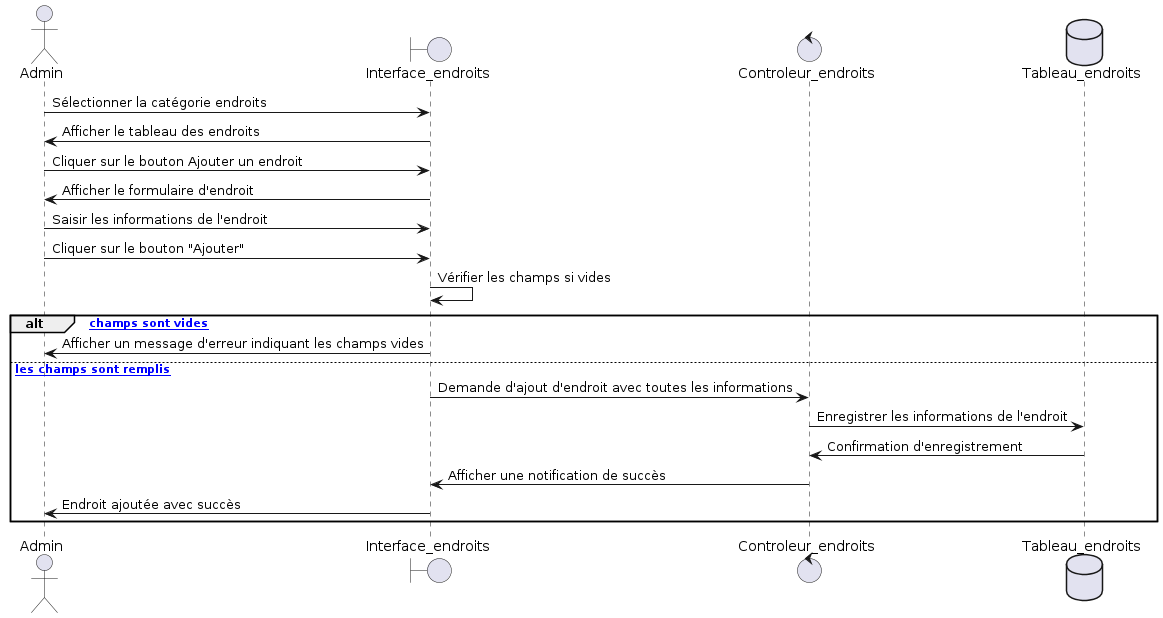
\includegraphics[height=13.5cm,width=15cm]{images/ffffajouterandroit.png}%
    }
    \caption{Figure du Diagramme de Séquence «Ajouter un Endorit» }
\end{figure}
\vspace{-1.2cm}
\subsection{Diagramme de séquence « Modifier un Endroit »}
\vspace{-4MM}
Le diagramme illustre le processus de modification d'un emplacement par l'admin sur la partie web de notre application.
\begin{figure}[H]%
    \center%
    \setlength{\fboxsep}{5pt}%
    \setlength{\fboxrule}{0.5pt}%
    \fbox{
    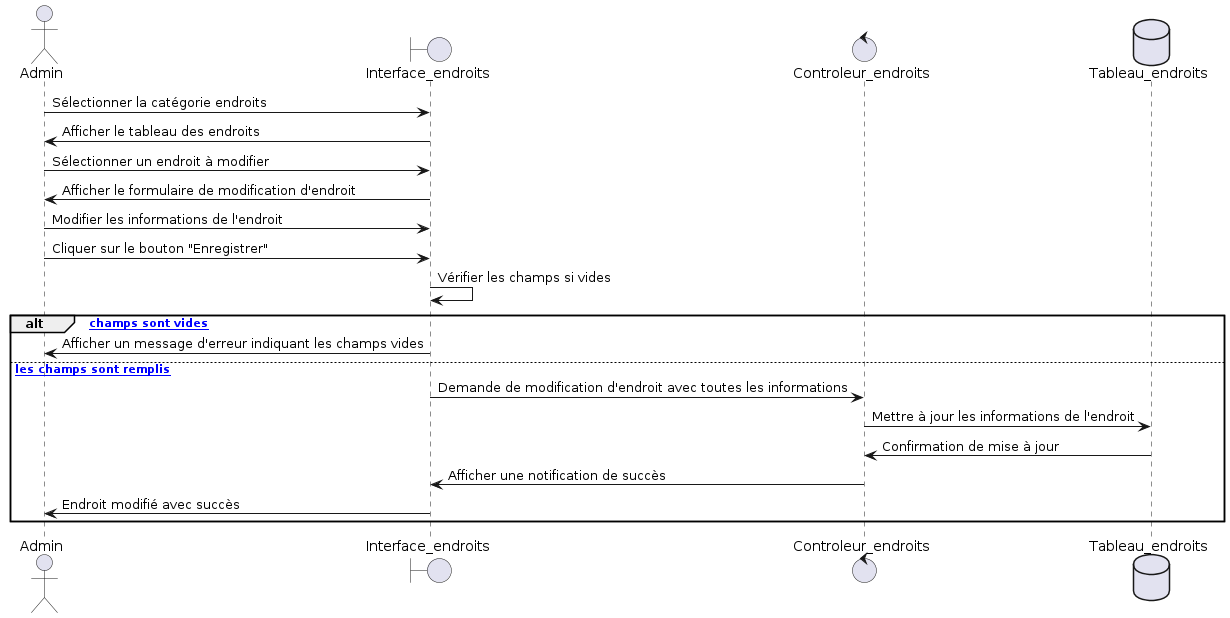
\includegraphics[height=9cm,width=15cm]{images/ffffeditendroit.png}%
    }
    \caption{Figure du Diagramme de Séquence «Modifier un Endroit» }
\end{figure}
\vspace{-1.2cm}
\subsection{Diagramme de séquence « Supprimer un Endroit »}
\vspace{-4mm}
Le diagramme représente l'action effectuée par l'admin sur la partie web de notre application pour supprimer un emplacement spécifique.

\begin{figure}[H]%
    \center%
    \setlength{\fboxsep}{5pt}%
    \setlength{\fboxrule}{0.5pt}%
    \fbox{
    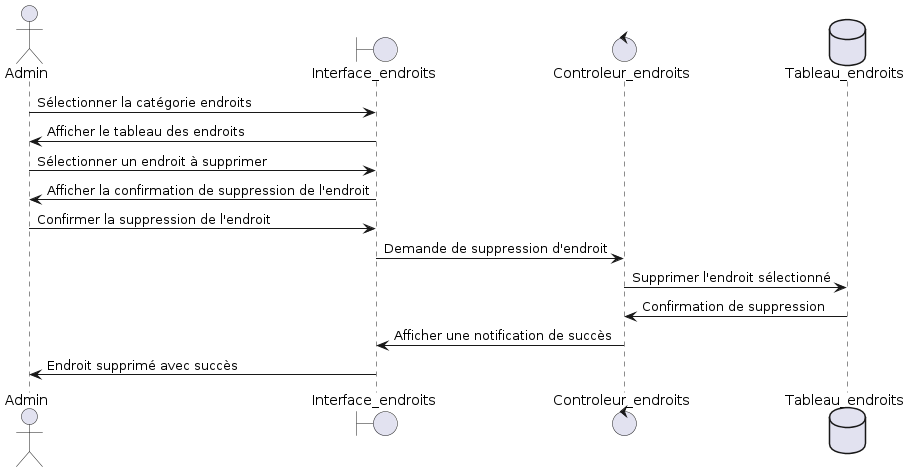
\includegraphics[height=9cm,width=15cm]{images/ffffsuppendroiy.png}%
    }
    \caption{Figure du Diagramme de Séquence «Supprimer un Endorit» }
\end{figure}
\newpage

\section{Diagramme de classes }
\vspace{-4mm}
Le diagramme de classes ci-dessus représente la gestion des universités, des facultés et des examens dans notre système. Chaque entité est modélisée par une classe correspondante, décrivant ses attributs et méthodes associées. Cette conception permet de visualiser clairement la structure des données et les relations entre les différentes entités, facilitant ainsi le développement et la maintenance du système.
\begin{figure}[H]%
    \center%
    \setlength{\fboxsep}{5pt}%
    \setlength{\fboxrule}{0.5pt}%
    \fbox{
    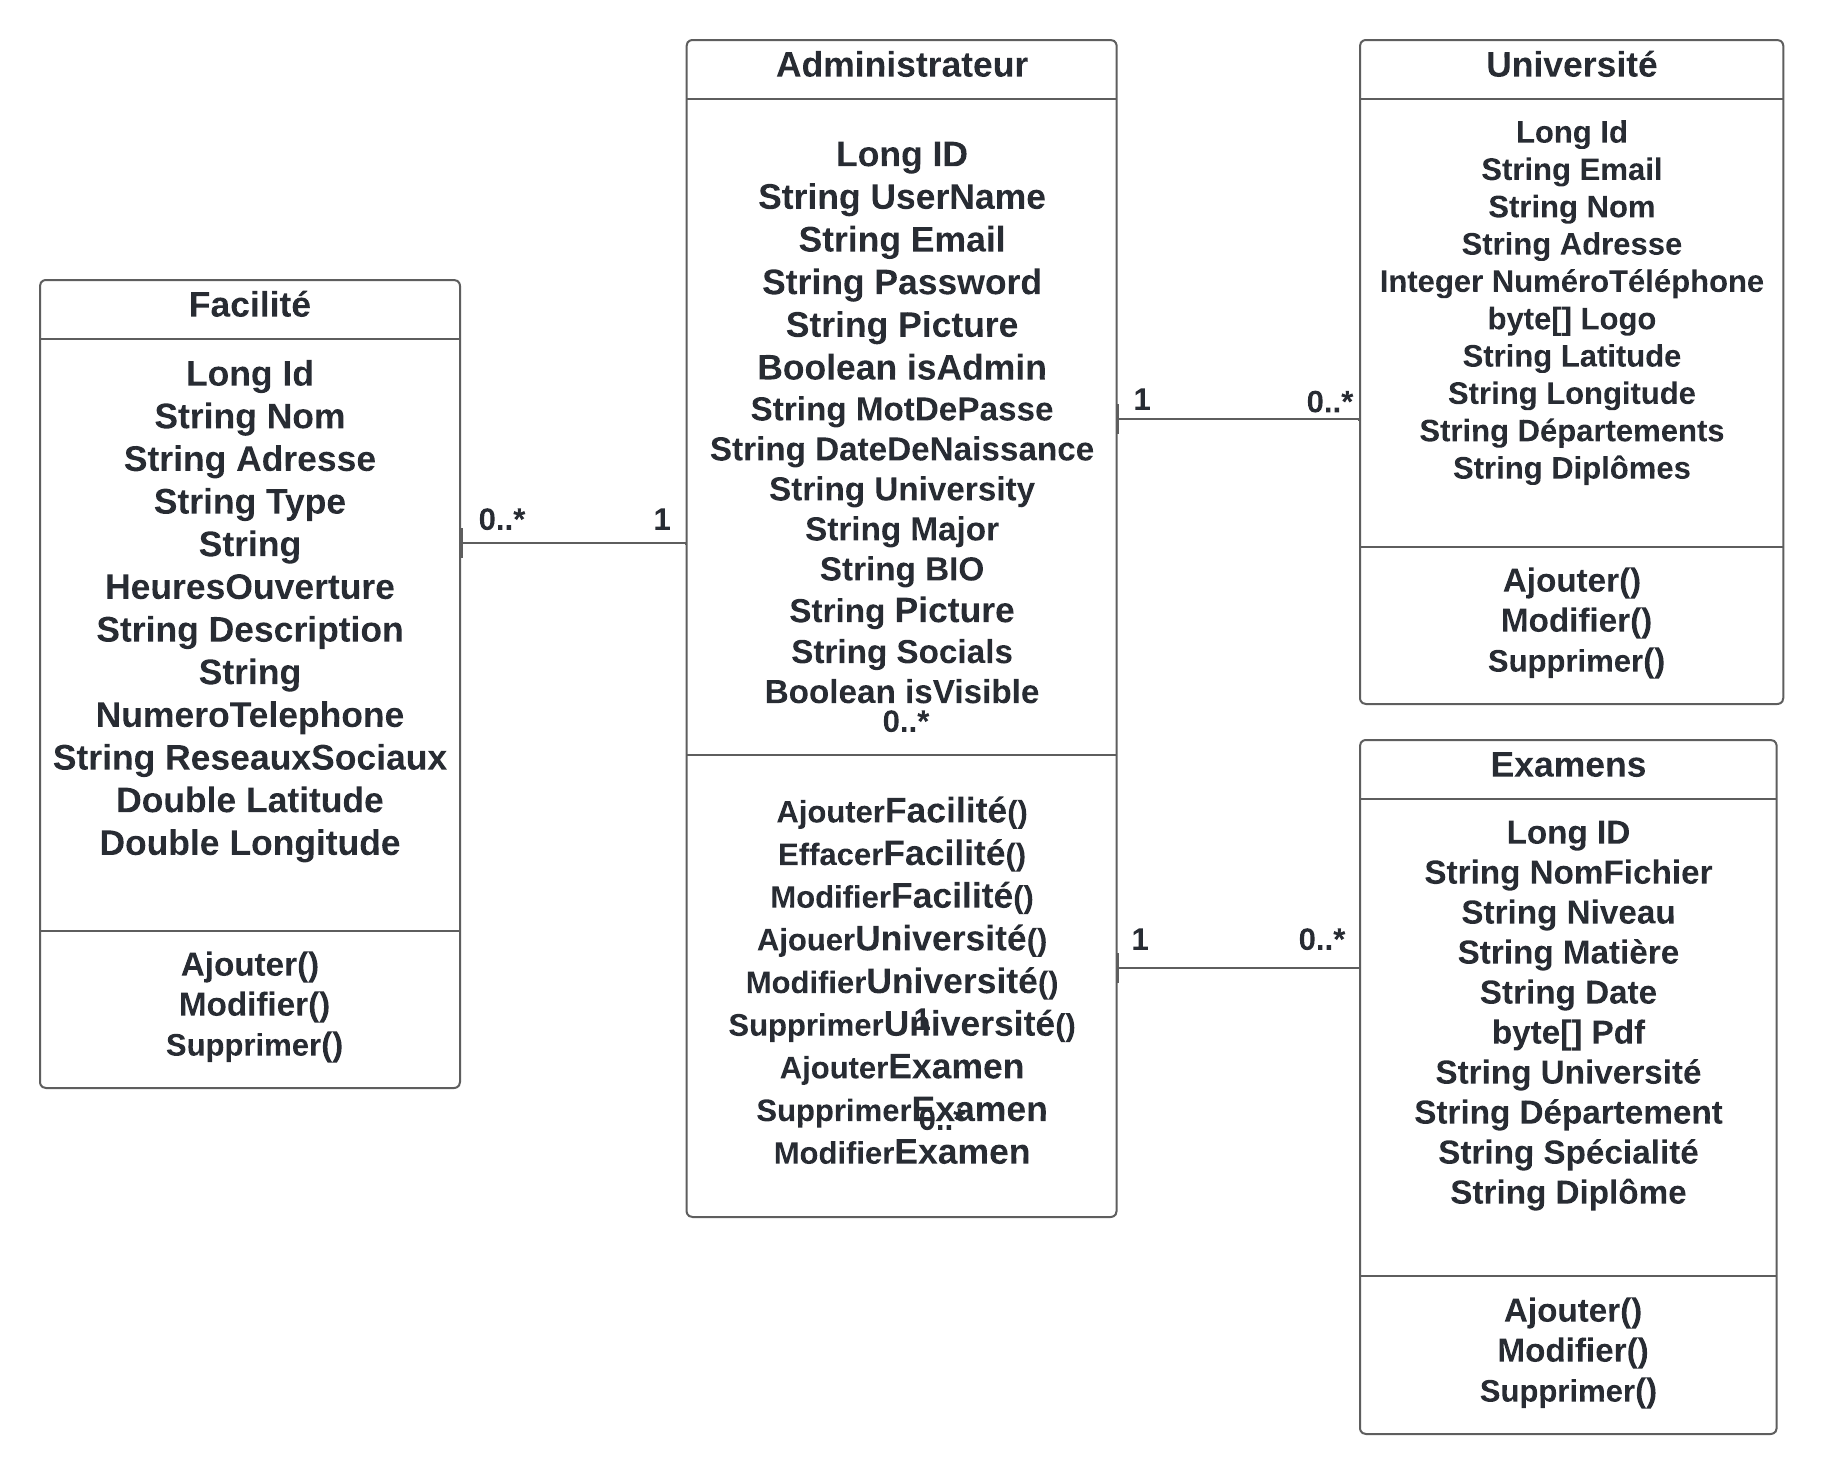
\includegraphics[height=17cm,width=15cm]{images/AAADiagramClassesUniExFac.png}%
    }
    \caption{Figure du Diagramme de classes de Sprint 2 }
\end{figure}

\section{Réalisation}
\vspace{-4mm}
La partie de réalisation représente la dernière phase du cycle de développement d’un sprint. Elle permet de présenter les résultats obtenus lors de l’étape de développement afin d’assurer et de garantir une version de qualité. Nous allons montrer cela par des captures d’écrans des fonctionnalités ayant été développées.
\vspace{-9Mm}
\subsection{Consultation de la liste des universités}
\vspace{-4mm}
L’interface d’ajout d'une université, c’est le premièr formulaire a remplir par l'admin .
\begin{figure}[H]%
    \center%
    \setlength{\fboxsep}{5pt}%
    \setlength{\fboxrule}{0.5pt}%
    \fbox{
    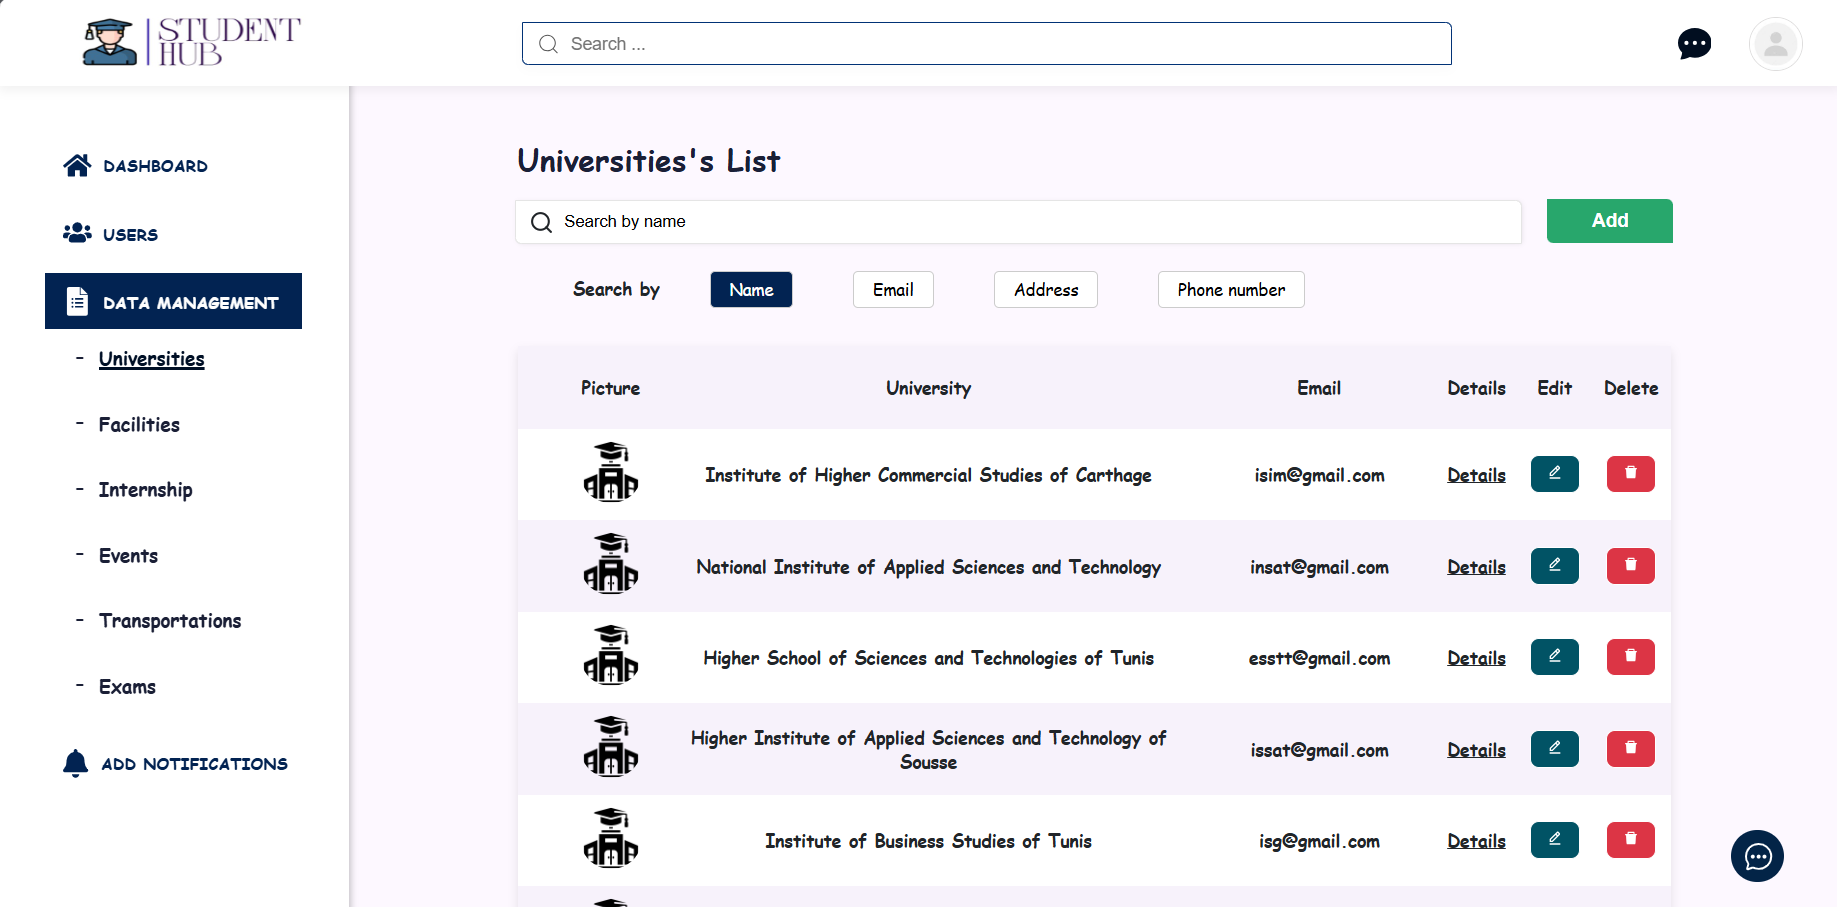
\includegraphics[height=14cm,width=16cm]{images/AAAUniversitiesPage.png}%
    }
    \caption{Interface Tableau des universités }
\end{figure}
\vspace{-1.2cm}
\subsection{Ajout d'une univesité}
\vspace{-4mm}
L’interface d’ajout d'une université, c’est le premièr formulaire a remplir par l'admin .
\vspace{-4mm}

\begin{figure}[htbp]
    \centering
    \setlength{\fboxsep}{5pt}%
    \setlength{\fboxrule}{0.5pt}%
    \fbox{
        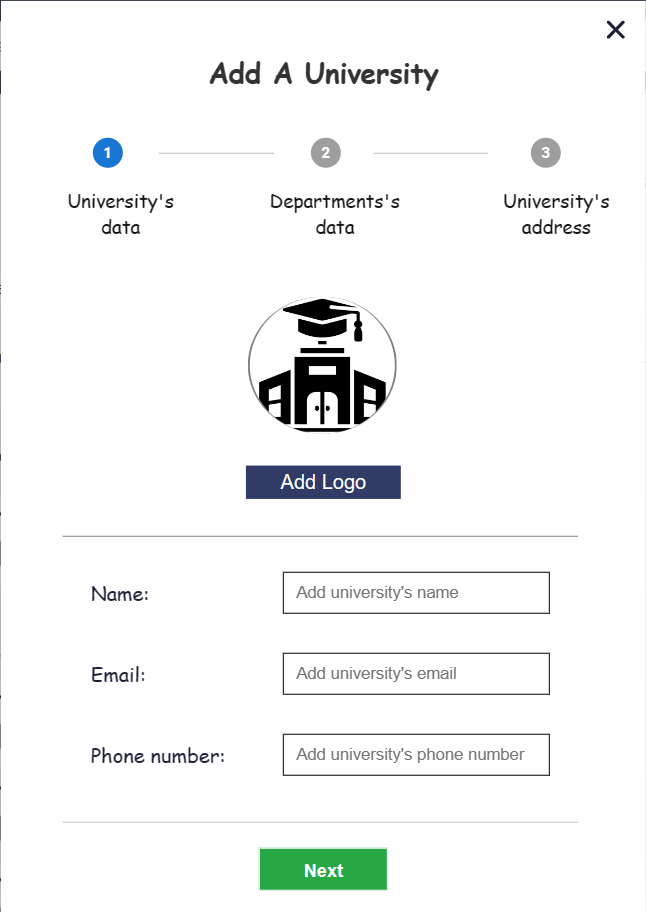
\includegraphics[height=7cm,width=12cm]{images/XAddUniversity1.png}
    }
    \label{fig:image1}
\end{figure}

\begin{figure}[htbp]
    \centering
    \setlength{\fboxsep}{5pt}%
    \setlength{\fboxrule}{0.5pt}%
    \fbox{
        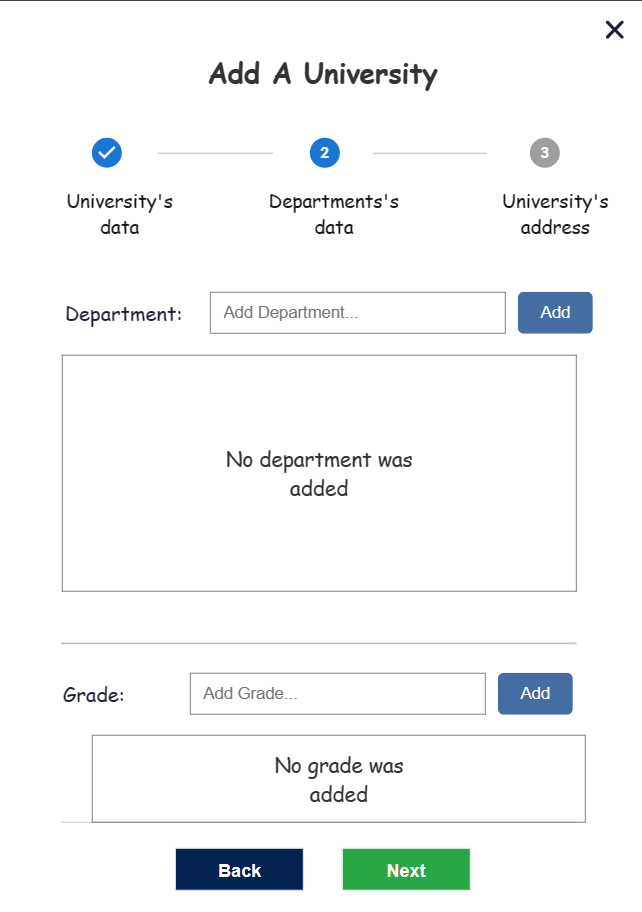
\includegraphics[height=7cm,width=12cm]{images/XAddUniversity2.png}
    }
    \label{fig:image2}
\end{figure}

\begin{figure}[htbp]
    \centering
    \setlength{\fboxsep}{5pt}%
    \setlength{\fboxrule}{0.5pt}%
    \fbox{
        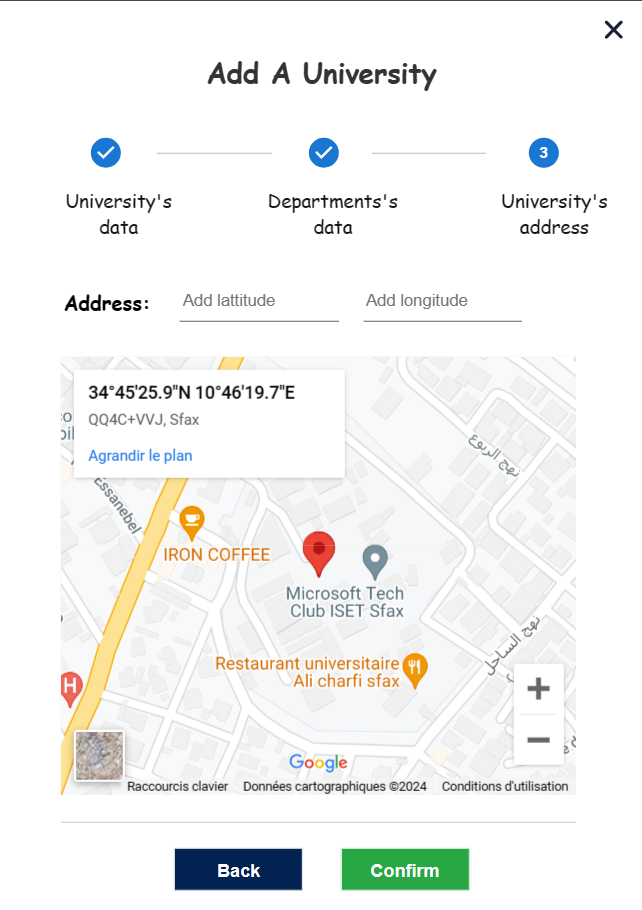
\includegraphics[height=7cm,width=12cm]{images/XAddUniversity3.png}
    }
    \caption{Interfaces d'ajout des universités}
    \label{fig:image3}
\end{figure}










\subsection{Modifier un endroit }
\vspace{-4mm}
interface de modification d'un endroit  par l'admin dans la base de données.
\vspace{-4mm}
\begin{figure}[H]%
    \center%
    \setlength{\fboxsep}{5pt}%
    \setlength{\fboxrule}{0.5pt}%
    \fbox{
    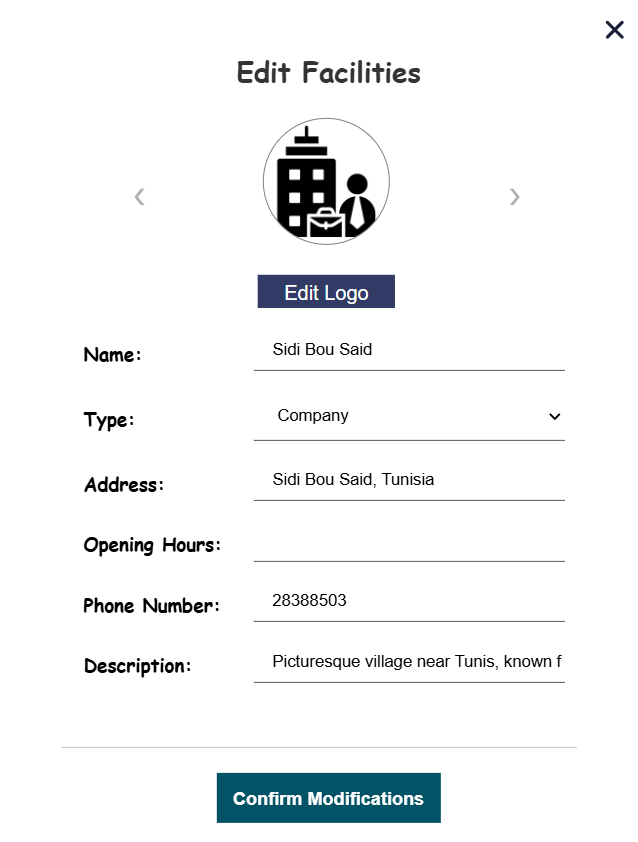
\includegraphics[height=8cm,width=12cm]{images/AAAEditFacility.png}%
    }
    \caption{Interface de modification d'un endroit  }
\end{figure}
\vspace{-1.2cm}
\subsection{Détails d'un examen}
\vspace{-4mm}
L'ad a la possibilité de consulter les détails des examens. Il peut afficher les examens directement sur le serveur sans les télécharger. De plus, l'admin peut également télécharger les examens sur son appareil si nécessaire.
\vspace{-2mm}
\begin{figure}[H]%
    \center%
    \setlength{\fboxsep}{5pt}%
    \setlength{\fboxrule}{0.5pt}%
    \fbox{
    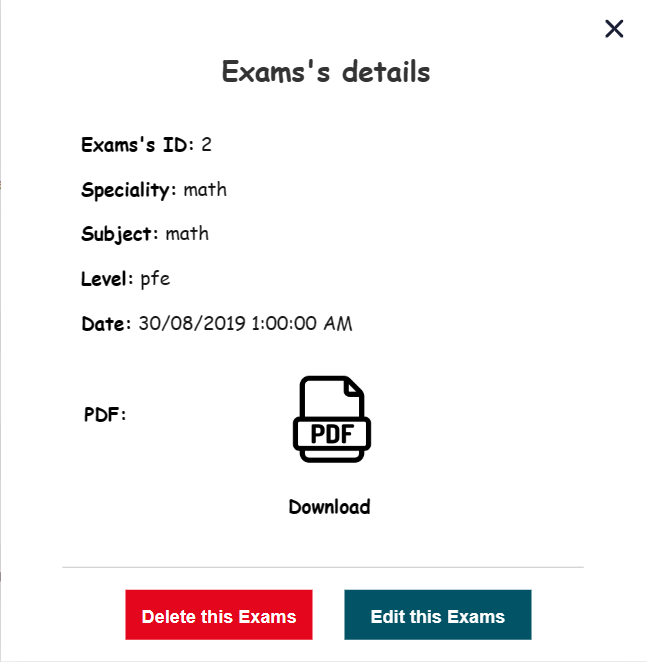
\includegraphics[height=8cm,width=12cm]{images/XExamsDetails.png}%
    }
    \caption{Interface de details d'un examen }
\end{figure}
\vspace{-4mm}
\newpage

\subsection{Détails Endroit dans l'application Mobile}
\vspace{-6mm}
L'interface "Détails Endroit" de l'appli mobile présente de façon détaillée les informations spécifiques d'un lieu, permettant aux utilisateurs d'accéder à toutes les données pertinentes.
\vspace{-4mm}
\begin{figure}[H]%
    \center%
    \setlength{\fboxsep}{5pt}%
    \setlength{\fboxrule}{0.5pt}%
    \fbox{
    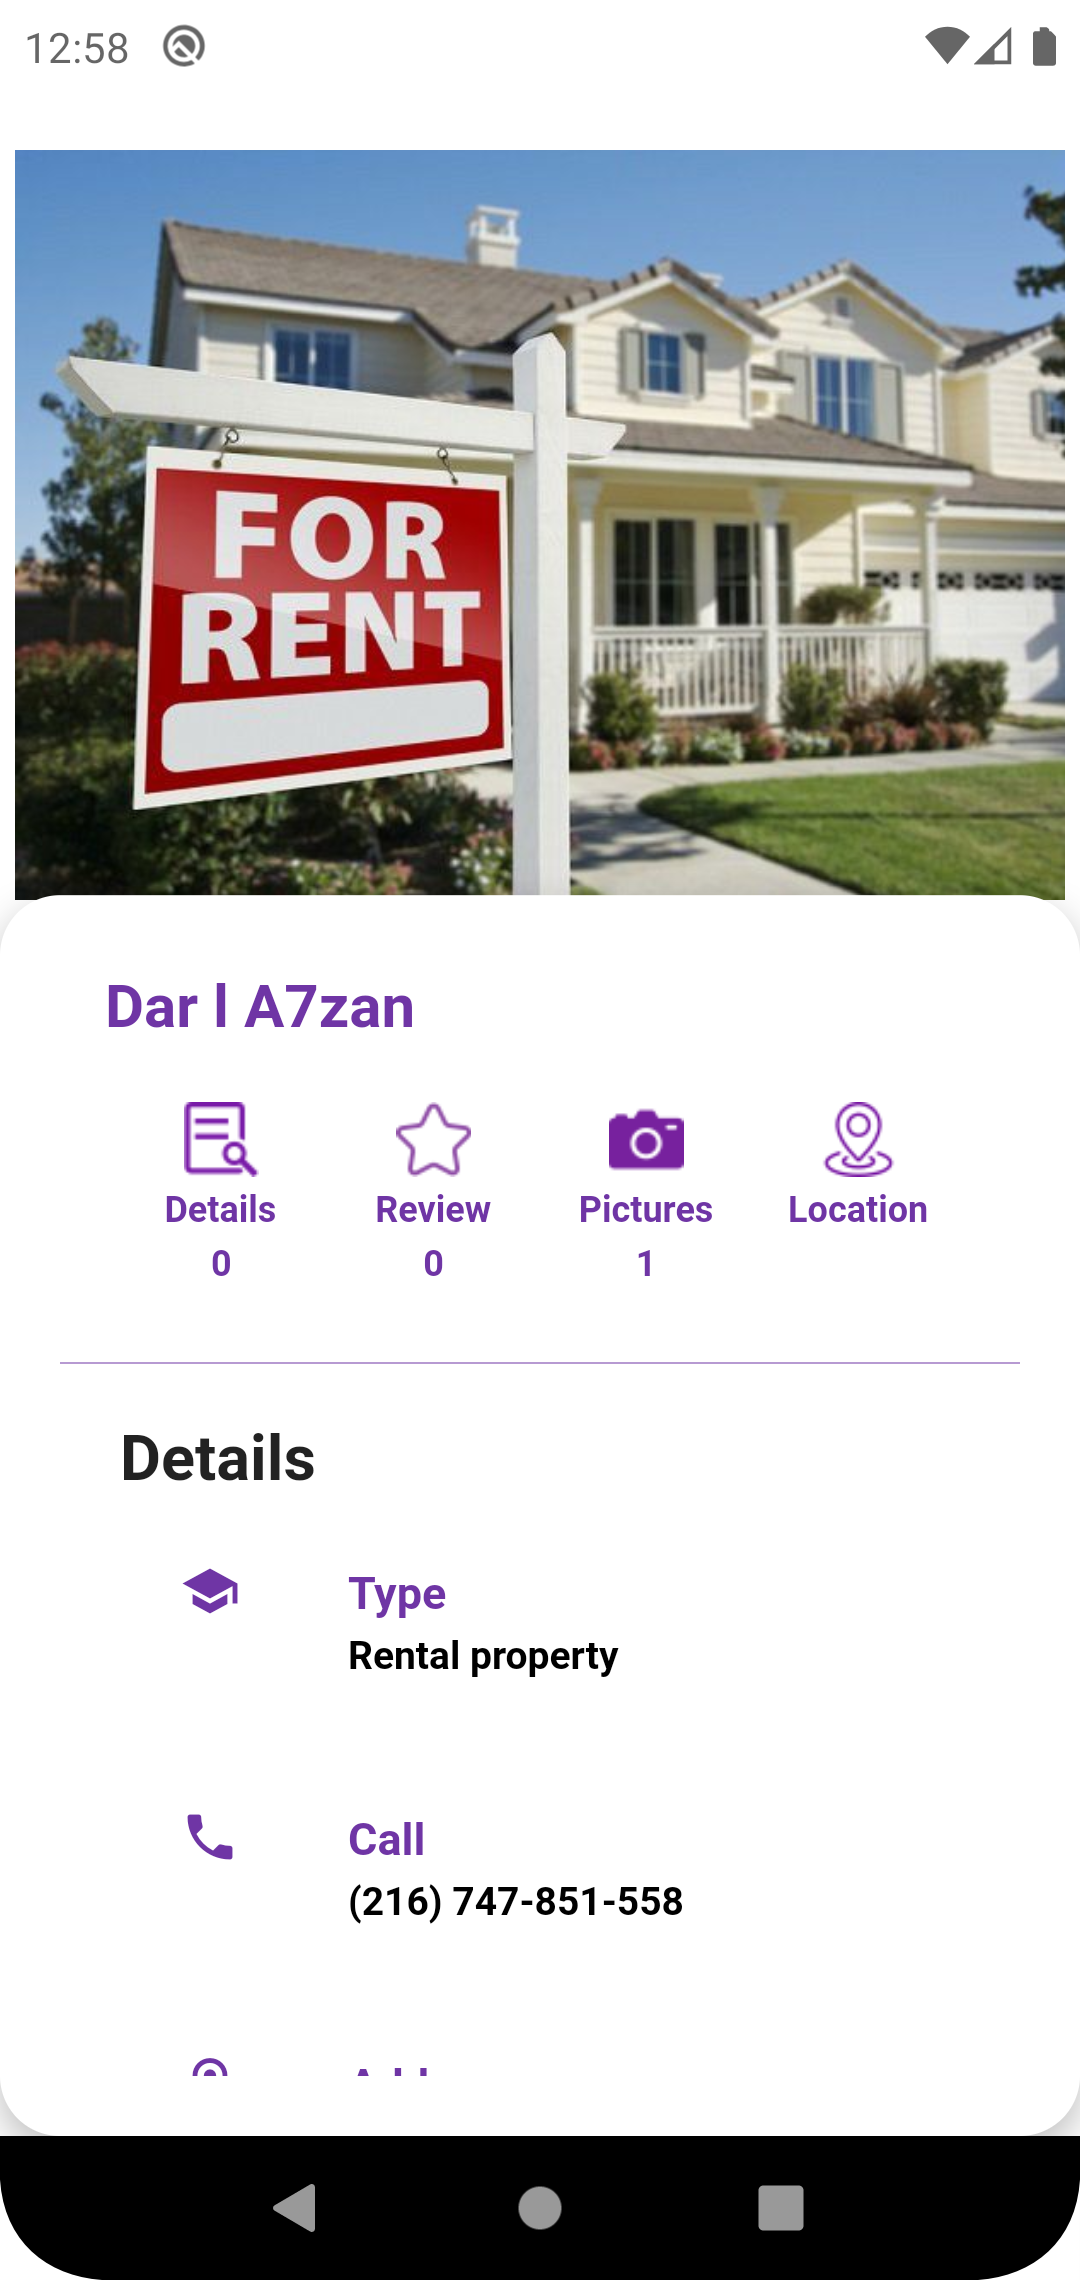
\includegraphics[height=9cm,width=7cm]{images/AAAFacilityDetails.png}
    }
    \caption{l'Interfaces d'endroit }
\end{figure}
\vspace{-1.8cm}
\subsection{Détails Université dans l'application Mobile}
\vspace{-6mm}
L'interface "Détails Université" de l'appli mobile fournit un aperçu complet d'une université.
\vspace{-4mm}
\begin{figure}[H]%
    \center%
    \setlength{\fboxsep}{5pt}%
    \setlength{\fboxrule}{0.5pt}%
    \fbox{
    
\includegraphics[height=9cm,width=7cm]{images/AAAUniversityDetails1.png}
    }
    \caption{l'Interfaces du page profile }
\end{figure}
\vspace{-1.8cm}
\subsection{Partie examen dans l'application mobile}
\vspace{-4mm}
IL'utilisateur de l'application mobile peut consulter les examens, les télécharger et les filtrer.

\begin{figure}[h]
    \centering
    \begin{minipage}[b]{0.45\linewidth}
        \centering
        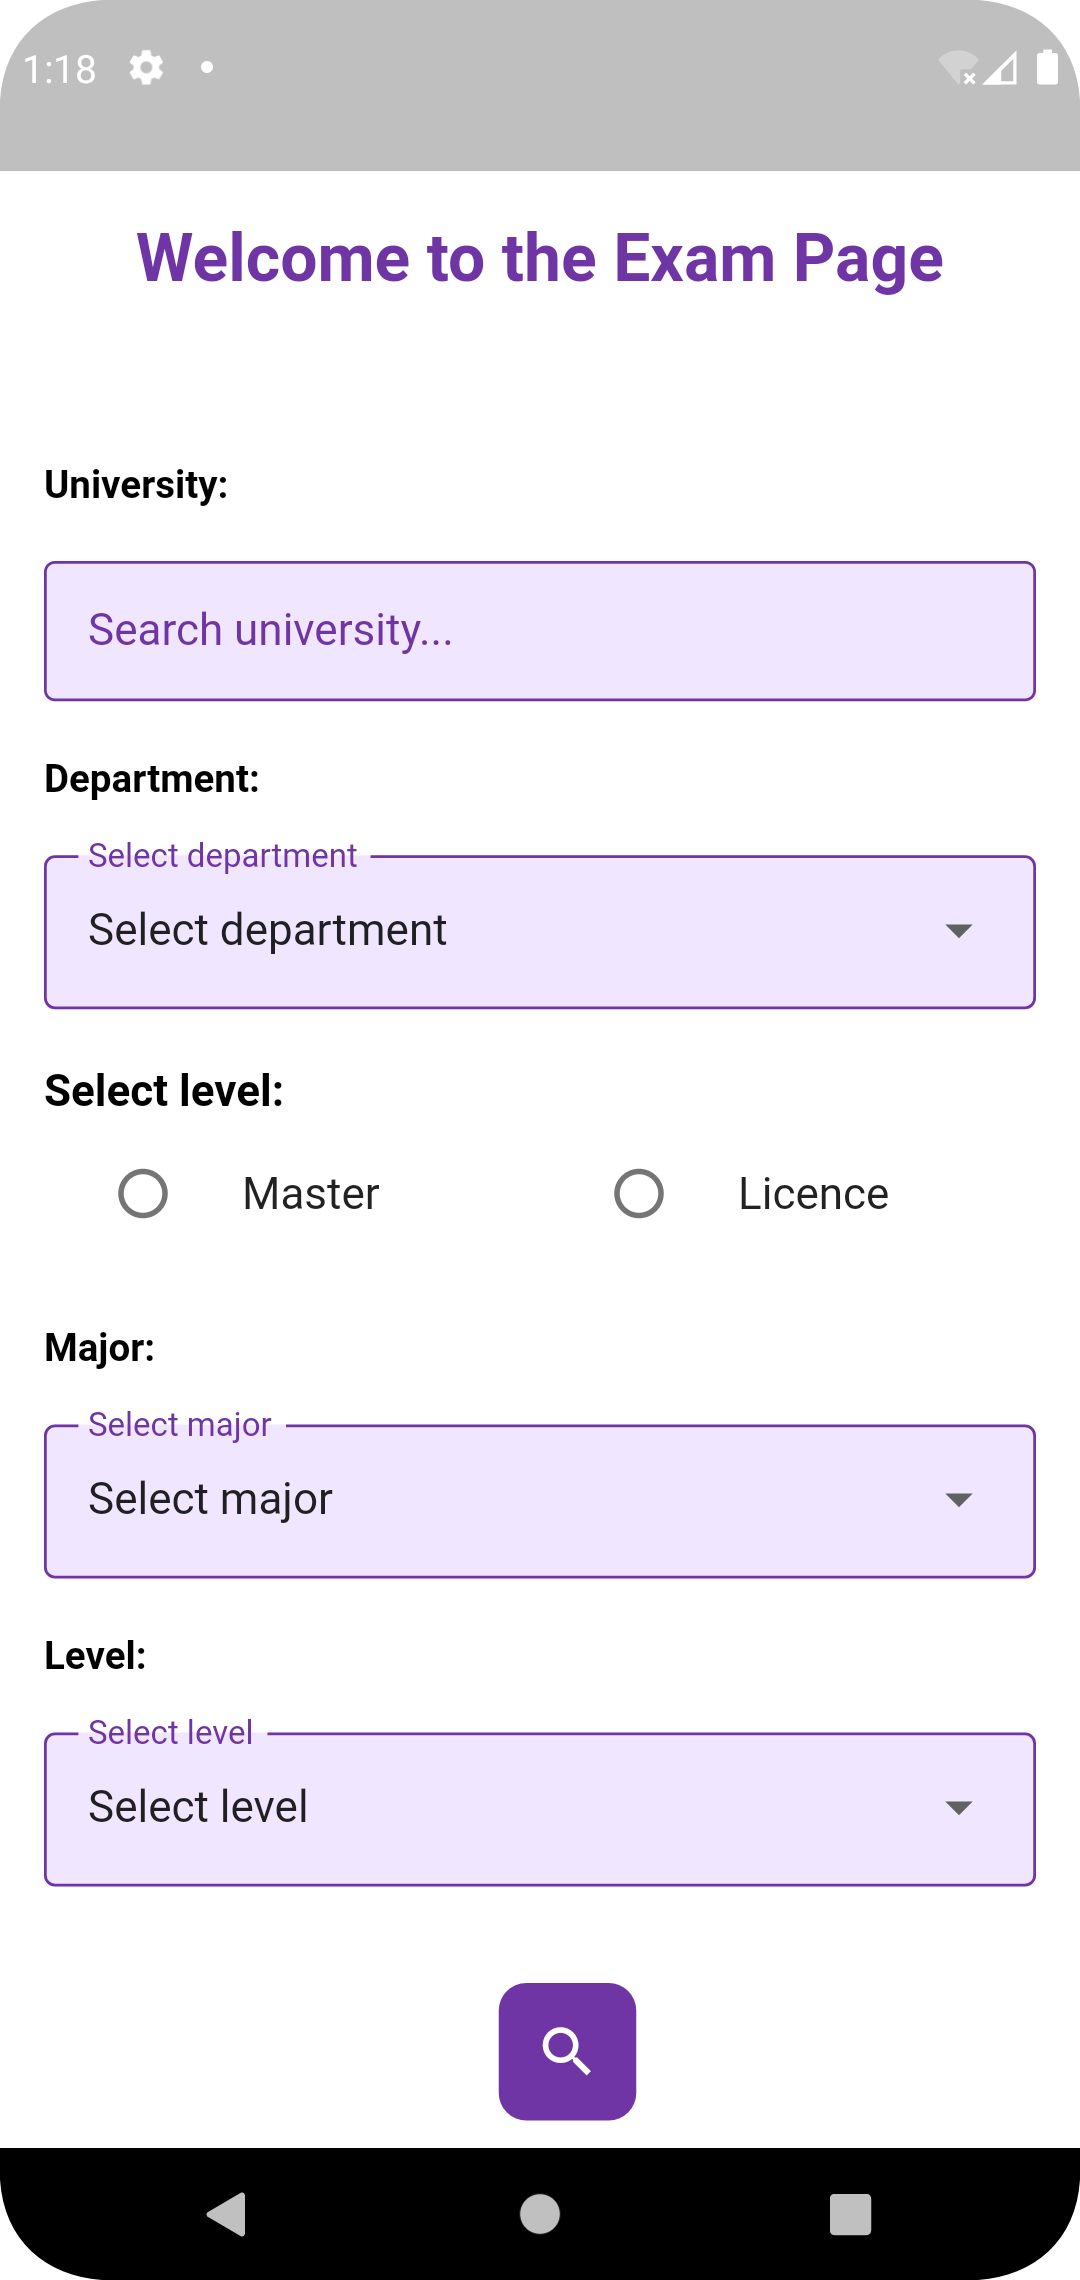
\includegraphics[height=10cm,width=7cm]{images/FilterExamsPage.png}
        \caption{Filtarage des examens}
        \label{fig:image1}
    \end{minipage}
    \hfill
    \begin{minipage}[b]{0.45\linewidth}
        \centering
        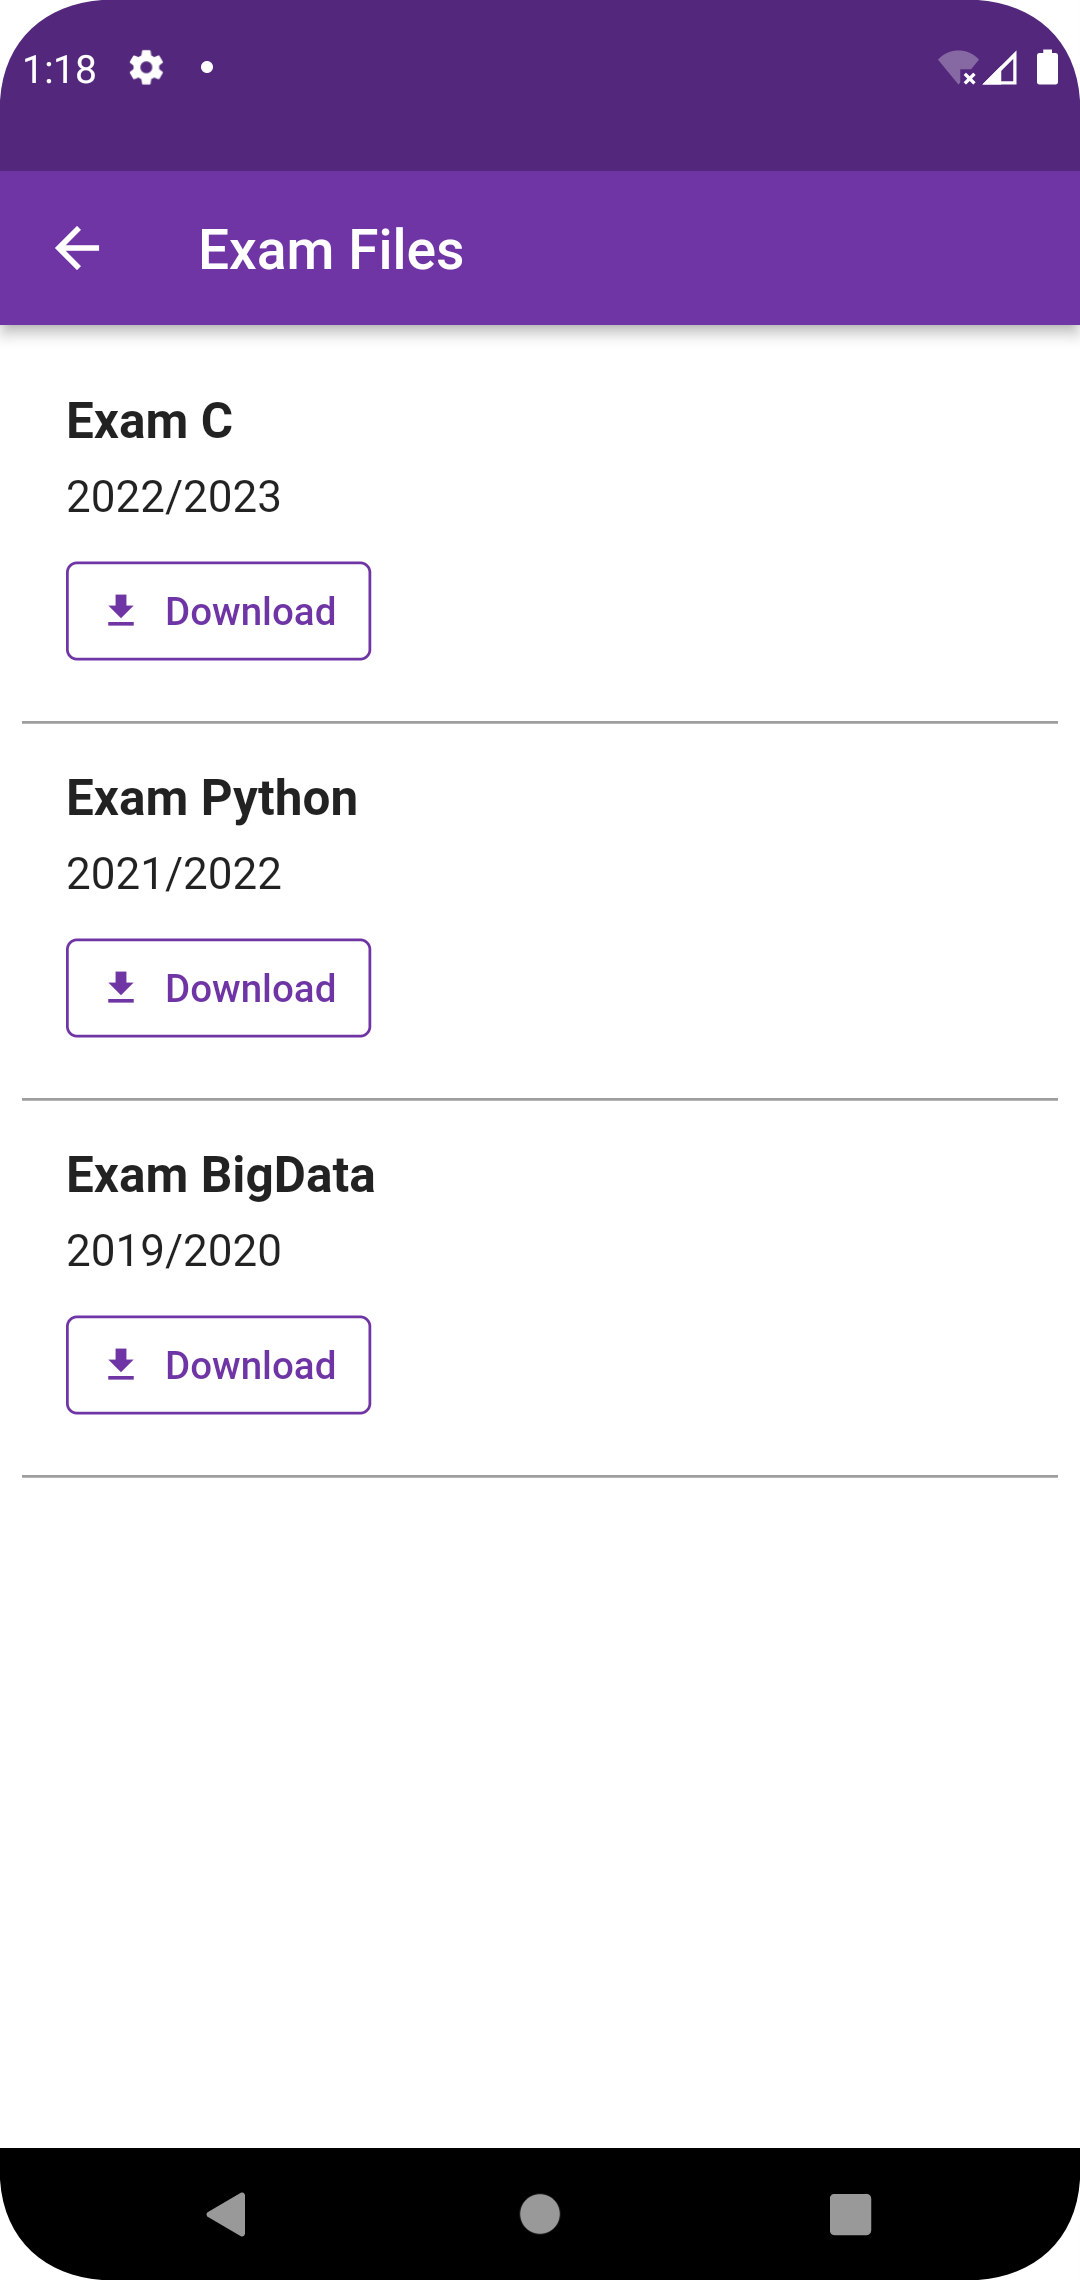
\includegraphics[height=10cm,width=7cm]{images/ExamsPage.png}
        \caption{List des exmanes \\
        }
        \label{fig:image2}
    \end{minipage}
\end{figure}
\vspace{-9mm}
\section{Conclusion }

En conclusion, ce sprint se concentre sur l'amélioration de la gestion des universités, des Endroits et des examens, afin de garantir une expérience utilisateur optimale sur l'application mobile. En dotant les admin d'outils sécurisés, nous visons à simplifier les processus admin, à assurer une gestion fluide des informations critiques et à offrir une visibilité claire et accessible des examens pour tous les utilisateurs. Ce sprint est une étape essentielle pour renforcer l'efficacité et la transparence de notre application.
\end{sloppypar} 
